\problemname{Desiigner strengir}

\illustration{0.35}{concert}{Mynd eftir \href{https://www.flickr.com/photos/benchun/8171429927/}{Ben Chun}}
% \begin{wrapfigure}{r}{0.35\textwidth}
%   \centering
%   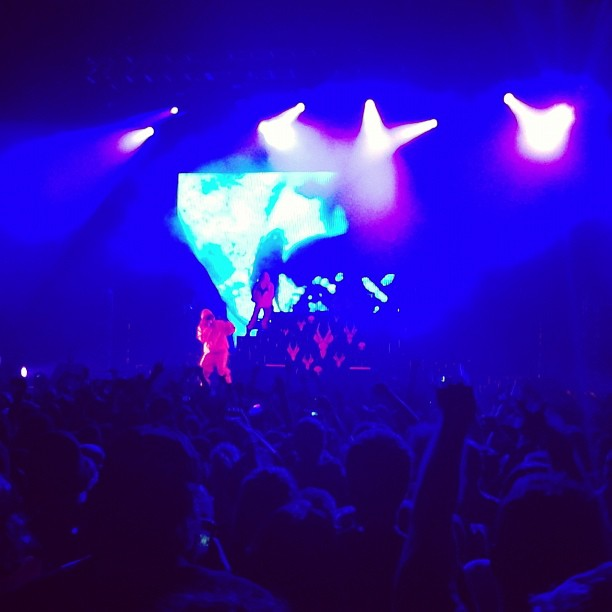
\includegraphics[width=0.93\textwidth]{concert.jpg}
% \end{wrapfigure}

Arnar fór nýlega á tónleika með fjölda rappara. Arnar uppgötvaði þar nýja
uppáhalds rapparann sinn, Desiigner. Því miður heyrði hann voða illa hvað
Desiigner var að segja, enda rappar hann mjög hratt og óskýrt. En hann heyrði
hann segja ákveðið orð nokkuð oft: það byrjar á stafnum `b', síðan komu tvö
eða fleiri eintök af stafnum `r', og að lokum var sérhljóði. Hann er ekki viss,
en það gæti til dæmis hafa verið orðið ``brra'' eða ``brrrru'', en klárlega ekki
``krrru'', ``ba'', ``bra'', né ``brrrt''. Og Arnar er meiraðsegja viss að enginn af
hinum röppurunum hafi sagt svona orð!

Núna langar Arnar að hlusta á lögin aftur, og það vildi svo heppilega til að
Unnar, vinur Arnars, var með myndavél á tónleikunum. Upptakan er því miður
óskýr, en rappið heyrist þó allavega vel.

Núna er Arnar að hlusta á eitt af lögunum, og hann heyrði eitthvað sem gæti
verið orð eins og Desiigner sagði. Er séns að þetta sé Desiigner? Hjálpaðu
Arnari að uppgötva ást sína á Desiigner með því að segja honum hvort orðið sem
hann heyrði sé Desiigner orð eða ekki.

\section*{Inntak}
Fyrsta og eina lína inntaksins er strengur sem inniheldur aðeins enska
lágstafi, og hefur lengd $n$ sem er í mesta lagi $10^3$.

\section*{Úttak}
Ef strengurinn er Desiigner strengur, þá á að skrifa út ``Jebb'', annars ``Neibb''.
Strengur er Desiigner strengur ef hann byrjar á bókstafnum `b', hefur svo
tvö eða fleiri eintök af bókstafnum `r', og endar svo á sérhljóða. Sérhljóðar
eru bókstafirnir `a', `e', `i', `o', `u' og `y'.

\section*{Útskýring á sýnidæmum}
Í fyrsta sýnidæminu er niðurstaðan ``Neibb'' því fjöldi `r' í strengum eru færri en 2.
Í öðru sýnidæminu er niðurstaðan ``Neibb'' því það eru fleiri en einn sérhljóði
í lokin. Í þriðja sýnidæminu er niðurstaðan ``Jebb'' því strengurinn er á því
formi sem beðið er um.

\section*{Stigagjöf}
Lausnin mun verða prófuð á miserfiðum inntaksgögnum, og er gögnunum skipt í
hópa eins og sýnt er í töflunni að neðan. Lausnin mun svo fá stig eftir því
hvaða hópar eru leystir.

\begin{tabular}{|l|l|l|l|}
\hline
Hópur & Stig & Inntak & Önnur skilyrði \\ \hline
1     & 50 & $n \geq 4$ & Strengurinn mun alltaf enda á bókstafnum `a'\\ \hline
2     & 40 & $n \geq 4$ & \\ \hline
3     & 10 & $n \geq 0$ & \\ \hline
\end{tabular}
